\section{Specification}
The algorithm for computing the MRI Q matrix, shown in Fig.~\ref{fig-1}. The main accelerating direction is to unroll the for-loops. The programmer view algorithm C code and input data set come from the Parboil benchmark suite~\cite{Rub1}.


%% In case you need to insert one or multiple figures with more complex layout,
%% you can use minipage. Save it to PDF and use the following
%% code. Remember to push the figure to the repository!
%% You can refer to a figure in the text with Fig.~\ref{fig:my_lable}
%% The letter in square brackets determines the position with respect to the
%% page: t=top; b=bottom; h=here
%% Change the minipage or the box width to adjust the size and the margins.
%% \begin{figure}[t]
%%   \begin{minipage}{\linewidth}
%% \centering
%%     \resizebox{\textwidth}{!}{
%%       \includegraphics{<path to figure>}
%%     }
%%   \end{minipage}
%%   \caption{Add a caption}
%%   \label{fig:my_label}
%% \end{figure}

\subsection{Assessment}
The goal of the assessment is to return correct Q matrix implemented on FPGA and compare the executing time of CPU and the accelerator designed. Also, several different designs will be implemented on FPGA to explore the design space.

\subsection{Milestones}\label{sec:arch}
\label{sec:milestones}

\vspace{-0.1in}
\begin{enumerate}
\setlength\itemsep{-0.15em}
  \item Analysis of the algorithm and the programmer's implementation in C (by Feb. 19)-- Done!
  \item Learning two tutorials: "How to design an accelerator in SystemC (Cadence Stratus HLS)" and "How to design a single-core SoC"\cite{esp1}. (by Feb. 28) -- Done!
  \item High-Level-Synthesis implementation in SystemC (by Mar. 11)-- Done!
  \vspace{-2mm}
       \begin{itemize}
            \item Transform programmer view algorithm to HLS-ready SystemC
            \item Initial HLS using the Cadence Stratus tool
       \end{itemize}

  \item Evaluation on an FPGA platform (by Mar. 25)
  \item Mid-term presentation and report (by Mar. 25)
  \item Initial Design Space Exploration (by Apr. 15)
  \item Enhanced Design Space Exploration (by Apr. 22)
  \item Final refinement and analysis (by May 5)
  \item Final presentation ($\sim$ May 11) and report ($\sim$ May 15)
\end{enumerate}

\subsection{Critical Aspects}
\begin{enumerate}
\setlength\itemsep{-0.15em}
\item Implement sine and cosine functions in the innermost for-loop.
\item Try different methods of optimization to reduce latency or decrease area.
\end{enumerate}

\begin{figure}[t]
\centering
\captionsetup{justification=centering, format=hang}
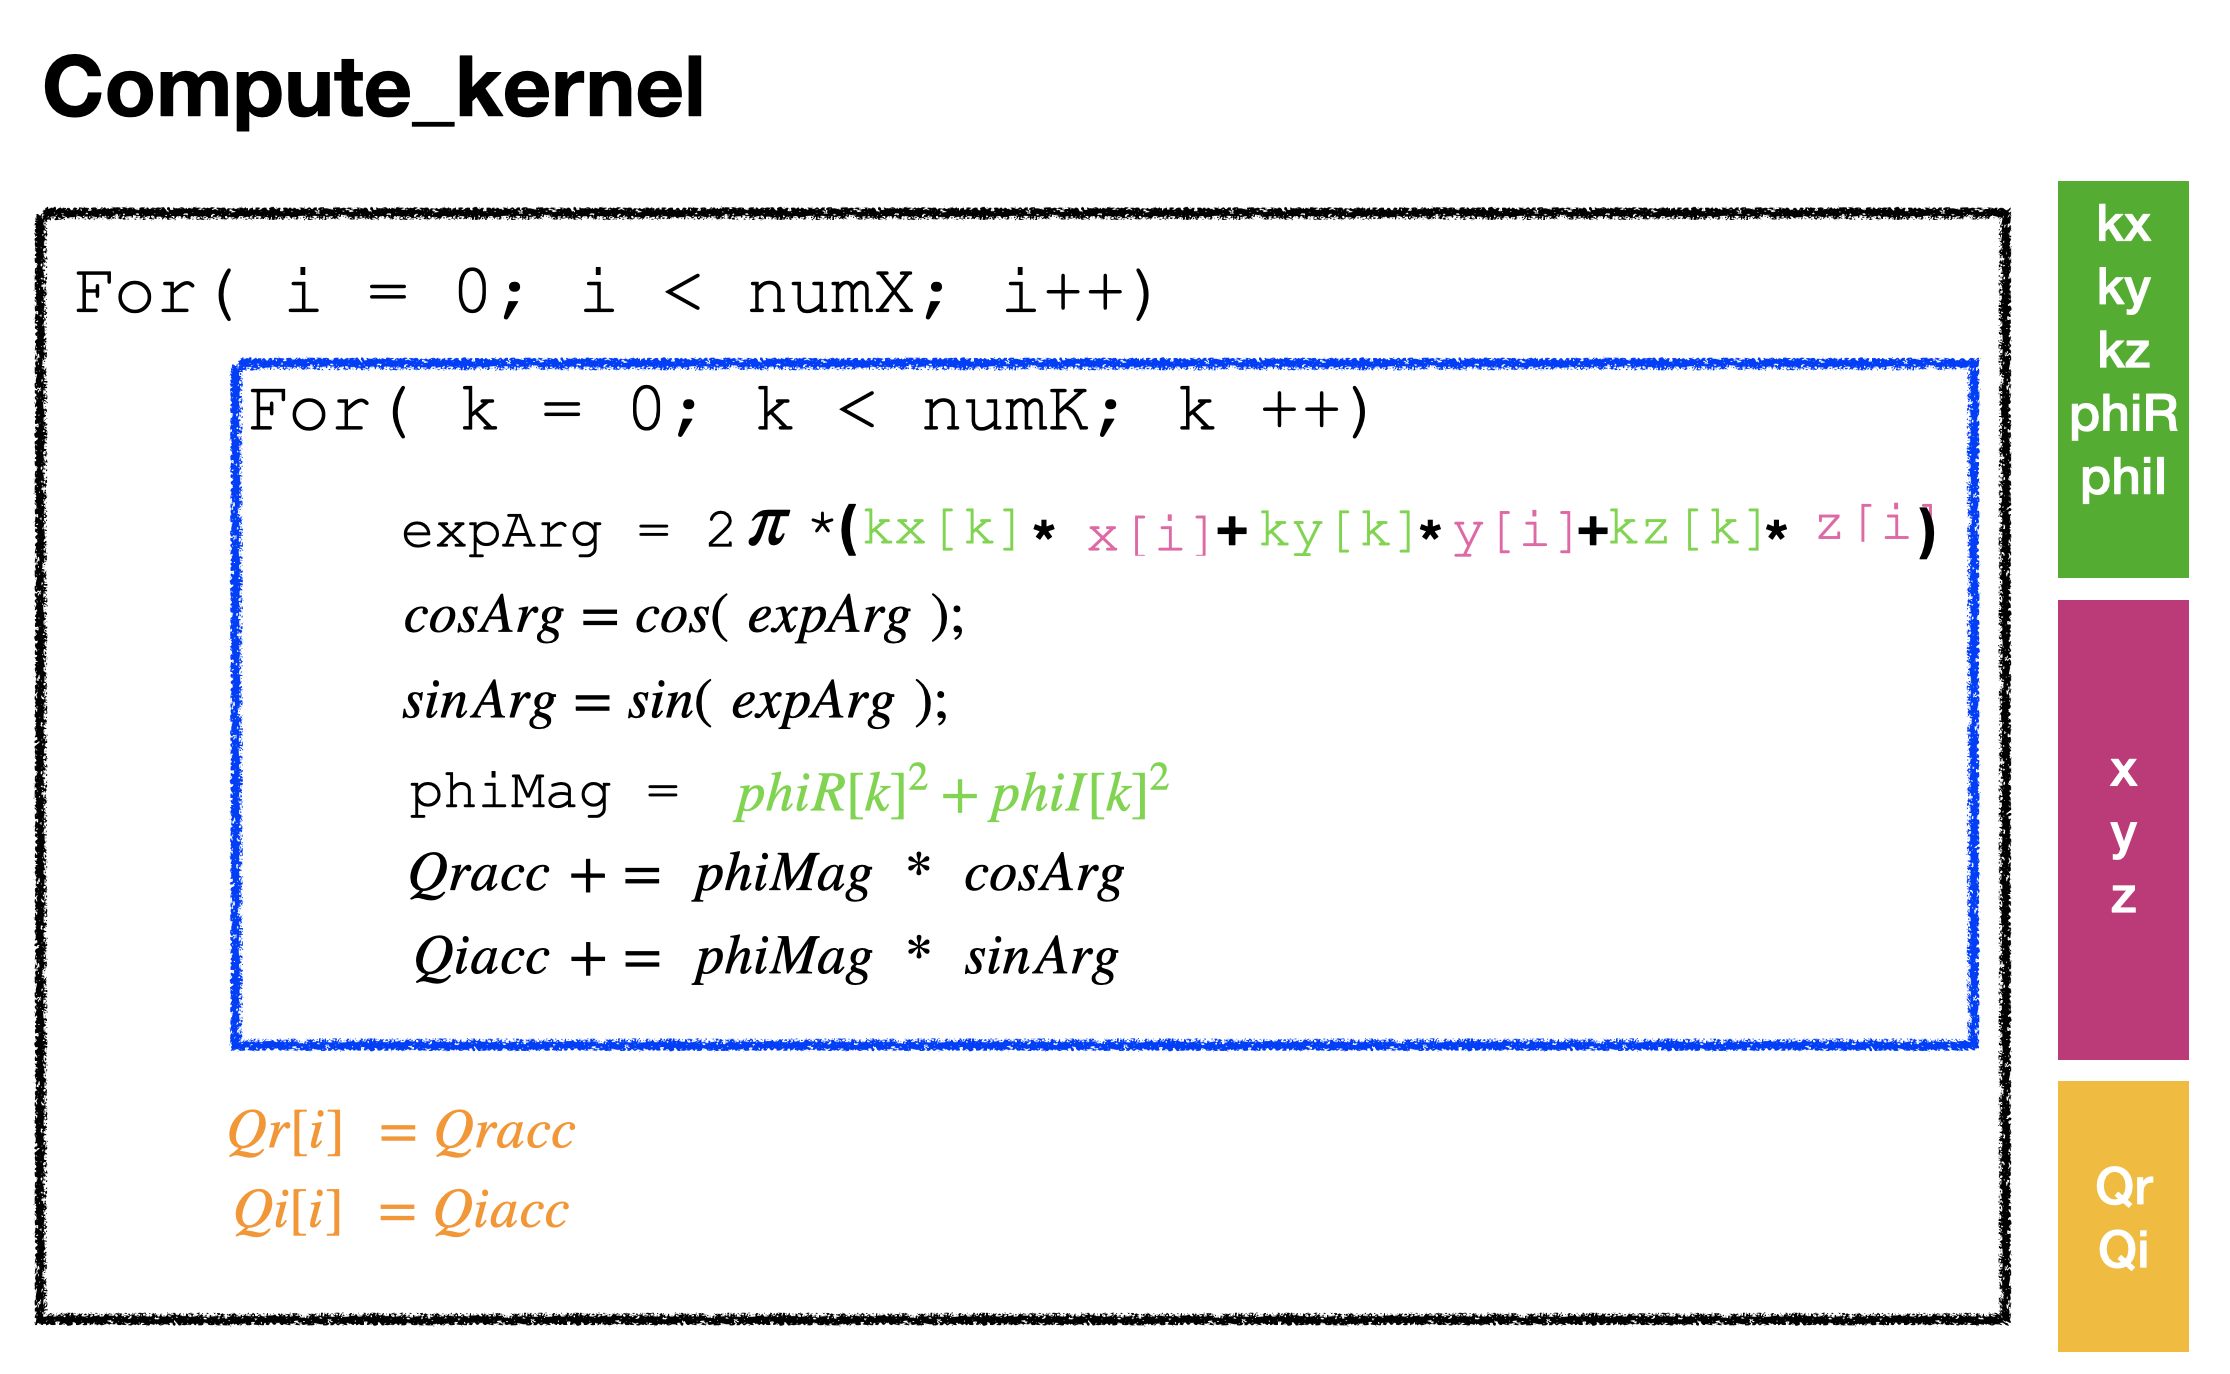
\includegraphics[width=0.85\columnwidth]{figures/algorithm.png}
\caption{Algorithm for computing MRI Q matrix~\cite{stone2008accelerating}}
\label{fig-1}
\end{figure}
